\documentclass{article}
\usepackage[utf8]{inputenc}
\usepackage{authblk}
\usepackage{natbib}
\usepackage{hyperref}
\usepackage{graphicx}
\usepackage{mathtools}                 % http://ctan.org/pkg/mathtools
\usepackage{amsmath}
\usepackage{listings}
\usepackage[a4paper, portrait, margin=1in]{geometry}

\usepackage[table]{xcolor}
\rowcolors{2}{gray!15}{white}
\newcommand{\head}[1]{%
   \textcolor{white}{\textbf{#1}}}
\renewcommand{\arraystretch}{1.5}

\title{\textbf{Analysis of 2-D Lid-Driven Cavity Problem}}
\author{Aakash Yadav\\ Email: \href{mailto:me16b001@iittp.ac.in}{me16b001@iittp.ac.in}}
\affil{\textbf{Indian Institute of Technology Tirupati}}
\date{\textbf{April 2019}}
\geometry{a4paper, portrait, margin=1in}

\begin{document}
\maketitle

\begin{center}
\line(1,0){250}
\end{center}

\begin{abstract}
The lid driven cavity problem is a very standard problem in domain of Computational Fluid Dynamics and is being used as a benchmark problem in CFD. The problem although appears to be simple , holds an ample opportunity for one to explore and has endless strings  attached to it.  The ultimate goal of this paper is to gain insight of some of the physics that is powering the modern CFD packages. In the current work, we present our analysis for both the steady  and unsteady states. We have used the derived variable approach for carrying out the analysis. For the steady state solutions, uniform grid has been used while for the unsteady state we have inplemented the non-uniform grid in order to capture the dynamics of the problem more accurately where the velocity gradients are very high. 
Accurate results inline with results obtained by Ghia et al \citep{ghia} have been obtained.
This paper also presents the methodolgy for Von-Neumann stability analysis in great depth. 
\end{abstract}

\section{Introduction}
% literature review regarding the usage of this problem
This problem has been solved by large numbers of people in the past by using different methodologies and schemes starting from 1966 by Burggraf \citep{burger}, yet it is an active area of research even in the present. Tamer et al \citep{tamer} provides a summary of all the work that has been done from 1966 till 2014 in very concise tabular format in chronological order.
The problem have been simulated upto Reynolds number, $Re=15000$ by Bruneau et al \citep{bruneau} in their 1990s paper by using a finite difference approach. It can be observed that Finite Difference scheme has been heavily adopted in the past for carrying out the analysis. In present work we have used the Finite Difference scheme for the unsteady state analysis while upwind scheme \citep{courant} (both first and second order) for the steady state analysis.

In this work, we have analyzed the unsteady, viscous, incompressible, isothermal, two-dimensional, laminar flow of Newtonian fluid taking place in the cavity, driven by lid of infinite length (Figure ~\ref{fig:cavityFig}). 
This problem is solved using an in-house Python code developed by the author (\href{https://github.com/AakashSYadav/LidDrivenCavityProblem}{https://github.com/AakashSYa dav/LidDrivenCavityProblem }), which solves both unsteady and steady  Navier-Stokes equations using derived variable apporach, using the Finite Difference Method (FDM).

The geometery of the problem is quite simple, it consists of a rectangular cavity ABCD in the $x-y$ plane with dimensions as shown in the Figure ~\ref{fig:cavityFig}, where the walls AB, CD, and AD are rigid walls, whereas BC is open. The cavity is of length, $D$ in the $x$-direction and height, $H$ in the y direction. The aspect ratio is defined as $r=H/D$. The Reynolds number is defined based on the velocity scale, $U$ and the length scale, $D$. Acceleration due to gravity acts in the negative $z$ direction. The top of the cavity, BC, is covered with an infinitely-long rigid lid. Initially $(t \leq 0)$, the fluid inside the cavity is at rest. At time $t > 0$, the lid is set in motion to the right with a constant velocity $U $. 

\begin{figure}[h!]
\centering
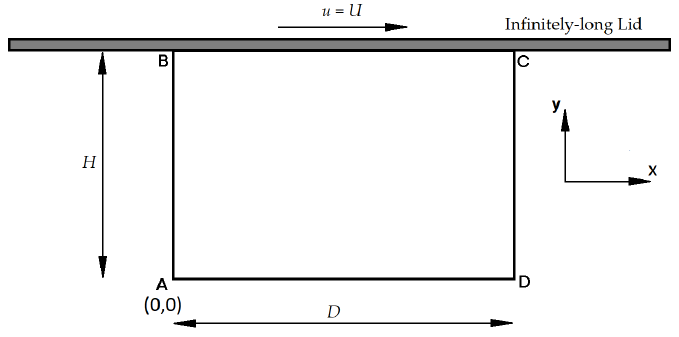
\includegraphics[scale=.5]{cavityFig.png}
\caption{Lid driven cavity in $x-y$ plane}
\label{fig:cavityFig}
\end{figure}

In section 2, we bring equtions governing the fluid flow in the appropriate form, the section that follows provides insights to boundary and initial conditions that are exisitng for this problem, and which can be used in solving the problem numerically. In section 4 and 5 we non-dimensionalise the governing equations and carry out their discretization in the later. Section 6, is the most important part of this paper which gives insight of the algorithm(s) used in this work. In the final section we present the conclusions. All the algorithms implemented in this work can be found in the appendix.

\section{Governing Equations}
\label{govEqn}
The equation of continuity for 2-D incompressible isothermal flow  \citep{Pedlosky, anderson1995computational} is given by the equation
\begin{equation}
\label{eqn:continuityEqn}
\frac{\partial u}{\partial x} + \frac{\partial v}{\partial y} = 0  
\end{equation}
where $u$ and $v$ are the components of veloity in $x$ and $y$ directions respectively. Furthermore we have the stream function, $\psi$ defined as

\begin{subequations}
\begin{equation}
\label{eqn:p1}
u = \frac{d\psi}{dy} 
\end{equation}
\begin{equation}
\label{eqn:p2}
v = -\frac{d\psi}{dx}
\end{equation}
\end{subequations}

The vorticity equation of fluid dynamics describes evolution of the vorticity $\omega$ of fluid as it moves with its flow, i.e. the local rotation of the fluid. Mathematically vorticity is the curl of the flow velocity.
\begin{subequations}
\begin{equation}
\label{eqn:w1}
\vec{\omega}^{\,} = \vec{\nabla}^{\,} \times \vec{V}^{\,}
\end{equation}
\begin{equation}
\label{eqn:w2}
\vec{\omega}^{\,} = (v_x - u_y)\hat{k}
\end{equation}
\begin{equation}
\label{eqn:streamFnEqn}
\vec{\omega}^{\,} = -\left[\frac{\partial^2 \psi}{\partial x^2} +  \frac{\partial^2 \psi}{\partial y^2}\right]=-\nabla^2 \psi
\end{equation}
\end{subequations}
Equation  ~\ref{eqn:streamFnEqn} can be obtained by combining equations ~\ref{eqn:p1}, ~\ref{eqn:p2} and \ref{eqn:w2}.

Navier-Stokes equations which follows are perhaps the most important equations in the field of Fluid Dynamics. These equations are essentially the momentum conservation equations for isothermal, Newtonian and incopressible fluid. This can also be seen as application of Isaac Newton's second law to fluid motion.
\begin{subequations}
\begin{equation}
\label{eqn:ns1}
\frac{\partial u}{\partial t} + u\frac{\partial u}{\partial x} + v\frac{\partial u}{\partial y}= -\frac{1}{\rho}\frac{\partial P}{\partial x} + g_x + \nu \left [ \frac{\partial^2 u}{\partial x^2} +  \frac{\partial^2 u}{\partial y^2} \right ]
\end{equation}

\begin{equation}
\label{eqn:ns2}
\frac{\partial v}{\partial t} + u\frac{\partial v}{\partial x} + v\frac{\partial v}{\partial y}= -\frac{1}{\rho}\frac{\partial P}{\partial y} + g_y + \nu \left [ \frac{\partial^2 v}{\partial x^2} +  \frac{\partial^2 v}{\partial y^2} \right ]
\end{equation}
\end{subequations}

Equations ~\ref{eqn:ns1} and ~\ref{eqn:ns2} are for the fluid flow along the $x$ and $y$ direction respectively.  One may observe that these equations also comprises of the pressure term $P$, which may not be required in some of the cases. We can eliminate the pressure term $P$ in order to reduce the number of variable and simplify the anylysis by computing $\frac{\partial (~\ref{eqn:ns1})}{\partial y} - \frac{\partial (~\ref{eqn:ns2})}{\partial x} $ , thus resulting in the below equation know as vorticity relation. This technique of approaching the problem is known as derived variable apporach. 
\begin{equation}
\label{eqn:vorticityFnEqn}
\frac{\partial \omega_z}{\partial t} + u\frac{\partial \omega_z}{\partial x} + v\frac{\partial \omega_z}{\partial y}= \nu \left [ \frac{\partial^2 \omega_z}{\partial x^2} +  \frac{\partial^2 \omega_z}{\partial y^2} \right ]
\end{equation}
% \notag

For the sake of convienance we will drop the subscript from the $\omega_z$ hereafter.




\section{Initial Conditions and Boundary Conditions}

At time $t=0$ everything is at rest and hence all the velocities, both of the fluid and the plate are zero. At the moment $t \geq0$ the lid will be moving at speed $u=U$, which will try to set the fluid in motion. We have the following boundary conditions for $t\geq0$ :
\\*
No slip condition will result in zero velocity along the wall tangent yields
\begin{subequations}
\begin{equation}
u(x,0)=0  \dots \text{ Bottom wall}
\end{equation}
\begin{equation}
v(D,y)=0 \dots \text{ Right wall}
\end{equation}
\begin{equation}
u(x,H)=U \dots \text{ Top wall}
\end{equation}
\begin{equation}
u(0,y)=0 \dots \text{ Left wall}
\end{equation}
\end{subequations}
\\*
While the no penetration condition that the walls of the cavity are impervious and impenetrable results into
\begin{subequations}
\begin{equation} 
v(x,0)=0 \dots \text{ Bottom wall}
\end{equation}
\begin{equation}
u(D,y)=0 \dots \text{ Right wall}
\end{equation}
\begin{equation}
v(x,H)=0 \dots \text{ Top wall}
\end{equation}
\begin{equation}
u(0,y)=0 \dots \text{ Left wall}
\end{equation}
\end{subequations}
More discussion of the boundary conditions will be followed in preceding section after their non-dimensionalization.

\section{Non-dimensionalization of the Governing Equations}
% comment on normalization	
In this section, we nondimensionalize the flow governing equations obtained in section \ref{govEqn}. This eases the analysis of the problem which, and reduces the number of free parameters, furthermore it helps to gain a greater insight into the relative size of various terms present in the equation. For carrying out non-dimensionalization we need appropriate scalings for the dimensionless variables, the scales are chosen for different quantites as shown below-
\begin{equation}
\hat{x}=\frac{x}{D}, \hat{y}=\frac{y}{H},  \hat{t}=\frac{U}{D}t,  \hat{u}=\frac{u}{U},  \hat{v}=\frac{v}{V_{ref}}, \hat{\psi}=\frac{\psi}{UD}, \hat{\omega}=\frac{\omega D}{U}
\end{equation}
\\*
We can obtain the scaling factor for the velocity in $y$ direction $v$ by carrying out non-dimensionalization of equation \ref{eqn:continuityEqn} which results into 
\begin{subequations}
\begin{equation}
\frac{U}{D}\frac{\partial \hat{u}}{\partial \hat{x}} + \frac{V_{ref}}{H}\frac{\partial \hat{v}}{\partial \hat{y}} = 0  
\end{equation}
\begin{equation}
\frac{U}{D}\sim \frac{V_{ref}}{H}  
\end{equation}
\begin{equation}
V_{ref}= \left(\frac{H}{D}\right)U = RU  
\end{equation}
\end{subequations}
Non-dimensionalising the stream function equation (\ref{eqn:streamFnEqn})
\begin{subequations}
\begin{equation}
\frac{\hat{\omega} U}{D} = -\left[\frac{\partial^2 (\hat{\psi}UD)}{\partial (\hat{x}D)^2} +  \frac{\partial^2 (\hat{\psi UD)}}{\partial (\hat{y}H)^2}\right]
\end{equation}
\begin{equation}
\label{eqn:streamFnEqn3}
\hat{\omega} = -\left[\frac{\partial^2 \hat{\psi}}{\partial \hat{x}^2} +  \frac{1}{r^2}\frac{\partial^2 \hat{\psi}}{\partial \hat{y}^2}\right]
\end{equation}
\end{subequations}
Non-dimensionalising the vorticity function equation (\ref{eqn:vorticityFnEqn})
\begin{subequations}
\begin{equation}
\frac{\partial \left(\frac{U}{D}\hat{\omega_z}\right)}{\partial \left(\frac{D}{U}\hat{t}\right)} + \hat{u}U\frac{\partial \left(\frac{U}{D}\hat{\omega_z}\right)}{\partial (\hat{x}D)} + \frac{UH}{D}\hat{v}\frac{\partial \left(\frac{U}{D}\hat{\omega_z}\right)}{\partial (\hat{y}H)}= \nu \left [ \frac{\partial^2 \left(\frac{U}{D}\hat{\omega_z}\right)}{\partial (\hat{x}D)^2} +  \frac{\partial^2 \left(\frac{U}{D}\hat{\omega_z}\right)}{\partial (\hat{y}H)^2} \right ]
\end{equation}
\begin{equation}
\frac{\partial \hat{\omega_z}}{\partial \hat{t}} + \hat{u}\frac{\partial \hat{\omega_z}}{\partial \hat{x}} + \hat{v}\frac{\partial \hat{\omega_z}}{\partial \hat{y}}= \frac{\nu}{UD} \left [ \frac{\partial^2 \hat{\omega_z}}{\partial \hat{x}^2} +  \frac{1}{r^2}\frac{\partial^2 \hat{\omega_z}}{\partial \hat{y}^2} \right ]
\end{equation}
\begin{equation}
\label{eqn:vorticityEqn2}
\frac{\partial \hat{\omega_z}}{\partial \hat{t}} + \hat{u}\frac{\partial \hat{\omega_z}}{\partial \hat{x}} + \hat{v}\frac{\partial \hat{\omega_z}}{\partial \hat{y}}= \frac{1}{Re} \left [ \frac{\partial^2 \hat{\omega_z}}{\partial \hat{x}^2} +  \frac{1}{r^2}\frac{\partial^2 \hat{\omega_z}}{\partial \hat{y}^2} \right ]
\end{equation}
\end{subequations}
Where, $Re = \frac{UD}{\nu}$, also we have 
\begin{equation}
\label{eqn:vorticityEqn3}
u=\frac{\partial \psi}{\partial y} , v=-\frac{\partial \psi}{\partial x} \notag
\end{equation}
\\*
Non-dimensionalisation of the above equation results into
\begin{equation}
\label{eqn:streamFnEqn2}
\hat{u}=\frac{1}{r}\frac{\partial \hat{\psi}}{\partial \hat{y}} , \hat{v}=-\frac{1}{r}\frac{\partial \hat{\psi}}{\partial \hat{x}}
\end{equation}
Substituting equation (\ref{eqn:streamFnEqn2}) in equation (\ref{eqn:vorticityEqn2}) yields 
\begin{equation}
\label{eqn:vorticityEqn4}
\frac{\partial \hat{\omega_z}}{\partial \hat{t}} +\frac{1}{r}\left[\frac{\partial \hat{\psi}}{\partial \hat{y}}\frac{\partial \hat{\omega_z}}{\partial \hat{x}} - \frac{\partial \hat{\psi}}{\partial \hat{x}}\frac{\partial \hat{\omega_z}}{\partial \hat{y}}\right]= \frac{1}{Re} \left [ \frac{\partial^2 \hat{\omega_z}}{\partial \hat{x}^2} +  \frac{1}{r^2}\frac{\partial^2 \hat{\omega_z}}{\partial \hat{y}^2} \right ]
\end{equation}
Deriving the boundary conditions in the form of vorticity and stream function
\begin{subequations}
\begin{equation}
\hat{\omega}(\hat{x},0) = - \frac{1}{r^2}\left(\frac{\partial^2 \hat{\psi}}{\partial \hat{y}^2}\right)_{\hat{y}=0} \dots \text{Bottom wall}
\end{equation}
\begin{equation}
\hat{\omega}(\hat{x},1) = - \frac{1}{r^2}\left(\frac{\partial^2 \hat{\psi}}{\partial \hat{y}^2}\right)_{\hat{y}=1} \dots \text{Top wall}
\end{equation}
\begin{equation}
\hat{\omega}(0,\hat{y}) = -\left(\frac{\partial^2 \hat{\psi}}{\partial \hat{x}^2}\right)_{\hat{x}=0} \dots \text{Left wall}
\end{equation}
\begin{equation}
\hat{\omega}(1,\hat{y}) = -\left(\frac{\partial^2 \hat{\psi}}{\partial \hat{x}^2}\right)_{\hat{x}=1} \dots \text{Right wall}
\end{equation}
\end{subequations}
We can expand $\psi$ using the Taylor series expansion as 
\begin{subequations}
\begin{equation}
\psi_{2,j} = \psi_{1,j}+\frac{\partial \psi}{\partial x}_{1,j}\Delta x + \frac{\partial^2 \psi}{\partial x^2}_{1,j}\frac{\Delta x}{2!} \dots
\end{equation}
\begin{equation}
\frac{\partial^2 \psi}{\partial x^2}_{1,j} = \frac{2(\psi_{2,j}-\psi_{1,j})}{\partial x^2} + \frac{2v_{1,j}}{\Delta x} +\mathcal{O}(\Delta x) 
\end{equation}
\end{subequations}
Similarly we can obtain the expressions as above for the other walls \citep{salih}.

For the bottom surface $\hat{u}=\hat{v}=0$, substituiting this equation (\ref{eqn:streamFnEqn2}) yields 
\begin{equation}
\hat{\psi}_{(\hat{y}=0)} = c_1
\end{equation}
Where $c_1$ is the constant of integration. Similarly we can obtain the equations for the other walls as
\begin{equation}
\hat{\psi}_{(\hat{x}=0)} = c_2, \hat{\psi}_{(\hat{x}=1)} = c_3 
\end{equation}
For the top wall we have 
\begin{equation}
\hat{u} = U =  \frac{1}{r}\frac{\partial \hat{\psi}}{\partial \hat{y}}  \Rightarrow \hat{\psi} = rUH+c_4  =c_5
\end{equation}
\begin{equation}
\hat{\psi}_{(\hat{y}=1)} = c_5
\end{equation}

\begin{figure}[h!]
\centering
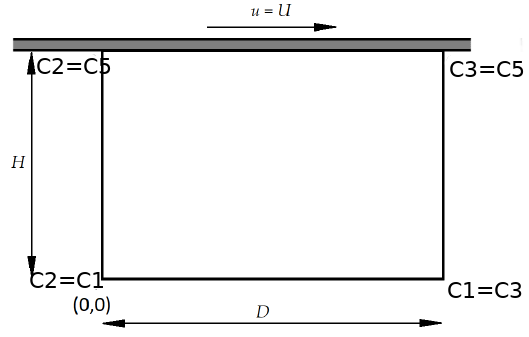
\includegraphics[scale=.4]{cavityFig2.png}
\caption{Continuity of the integration contants at the vertices}
\label{fig:cavityFig2}
\end{figure}

We can choose the constants to be equal to each other i.e.  $c_1=c_2=c_3=c_5=c$ because of the continuity at the corners as shown in the Figure \ref{fig:cavityFig2}. Without any loss of generality we can set $c=0$ as $\psi$ is a relative term.
Hence
\begin{equation}
\hat{\psi}_{(y=0)}=\hat{\psi}_{(y=1)}=\hat{\psi}_{(x=0)}=\hat{\psi}_{(x=1)}=0
\end{equation}




\section{ Discretization Schemes}
% comment why do we use such a grid with a stretching function --> velocity gradient is hight near walls. Why only that particular stretching function
In this section we focus on discretisation of the domain in smaller regions. This is inherently a two step process, first we meshing i.e. divide the domain into smaller regions. These smaller regions may be triangles and rectangles (in 2D) and tetrahedrons, hexahedrons (in 3D) and other types of geometric entities, but in our case we stick to the rectangular grids. The vertices of these geometric entities are called nodes. Secondly, we discretize the governing equations over the predefined mesh. In the analysis that follows we will drop the 'hat' notation for dimensionless variables for convienance. We present this process in to different subsections one each for steady (uniform grid) and unsteady state (non-uniform grid).

\subsection{Discretization for Non-uniform grid}
\begin{figure}[h!]
\centering
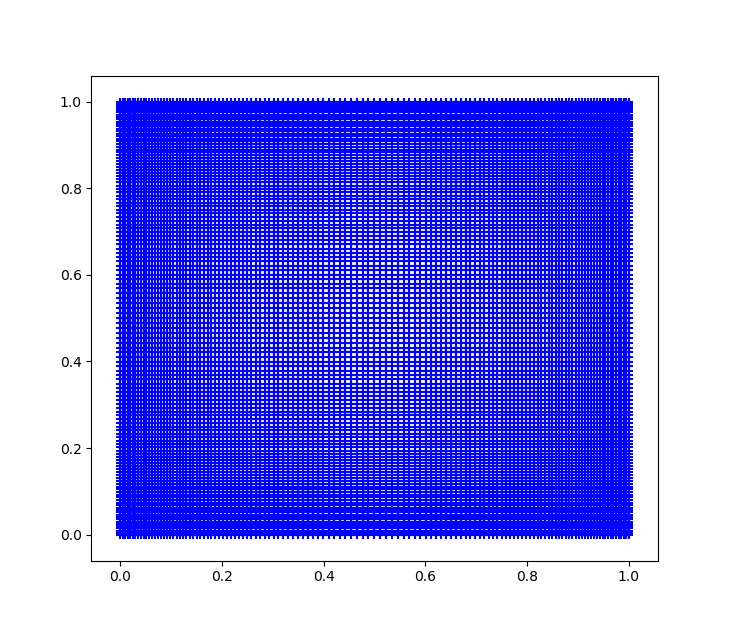
\includegraphics[scale=.5]{Figure_1.png}
\caption{A 128 $\times$ 128 Non-uniform grid generated by the program}
\label{fig:gridImage}
\end{figure}

We have used the Forward Time Central Space (FTCS) scheme for the non-uniform grid. The main reason for using the non-uniform grid is enable our analysis to capture accurately the dynamics near the walls where the velocity gradients are very high. The grid size is relatively bigger near the center in order to save some computaion time, also close to the center ther wont be any drastic changes. The non-uniform grid that is not equally spaced as shown in Figure \ref{fig:gridImage}. The grid has been obtained by using $tanh$ function, the grid stretching can be changed as required by supplying the stretching parameter $\gamma$ to the grid stretching function (see Appendix for implementaion). Function used for grid generation -  
\begin{equation}
y_j = 1- \frac{tanh\left[\gamma\left(1-\frac{2j}{N}\right)\right]}{tanh(\gamma)} \text{   }  j =1,2,3 \dots N
\end{equation}

\begin{figure}[h!]
\centering
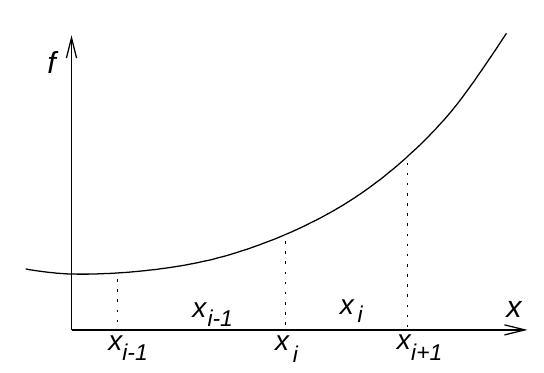
\includegraphics[scale=.4]{nugrid.png}
\caption{Non-unform spacing along the $x-$axis (Credit- Craft)}
\label{fig:nugrid}
\end{figure}
Now we derive the FTCS scheme for non-uniform grid. We use Taylor series expansions to develop and/or analyse the accuracy of numerical approximations for derivatives. Using Taylor series expansions for the grid point as shown in Figure \ref{fig:nugrid} we can write
\begin{subequations}
\begin{equation}
f(x_{i+1}) = f(x_i) + \Delta x_i f^{'}(x_i)+\frac{(\Delta x_i)^2}{2!}f^{''}(x_i)  + \frac{(\Delta x_i)^3}{3!}f^{'''}(x_i)  \dots
\end{equation}
\begin{equation}
f(x_{i-1}) = f(x_i) -\Delta x_{i-1} f^{'}(x_i)+\frac{(\Delta x_{i-1})^2}{2!}f^{''}(x_i)  - \frac{(\Delta x_{i-1})^3}{3!}f^{'''}(x_i)  \dots
\end{equation}
\end{subequations}
Using the above to equation we can discretized derivatives to be
\begin{subequations}
\begin{equation}
f^{'}(x_i) = \frac{f(x_{i+1})-f(x_{i-1})}{\Delta x_i + \Delta x_{i-1}} + \mathcal{O}(\Delta x)
\end{equation}
\begin{equation}
f^{''}(x_i) = \frac{\Delta x_{i-1} f(x_{i+1}) + \Delta x_{i}f(x_{i-1}) - (\Delta x_i + \Delta x_{i-1}f(x_i))}{\Delta x_{i-1}\Delta x_i +\Delta x_{i} \Delta x_{i-1}} + \mathcal{O}(\Delta x)
\end{equation}
\end{subequations}
Although, the equations appear to be only first order accurate for the non-uniform grid, they approach second order accuracy when the grid size are very close to each other i.e. the case of uniform grid. We can write the discretised form for the equation ~\ref{eqn:streamFnEqn3} and  ~\ref{eqn:vorticityEqn2} as 
\begin{subequations}
\begin{equation}
\begin{split}
\label{eqn:main1}
-\omega_{ij} =2\left[\frac{\Delta x_{i-1} \psi(x_{i+1}) + \Delta x_{i}\psi(x_{i-1}) - (\Delta x_i + \Delta x_{i-1}\psi(x_i))}{\Delta x_{i-1}\Delta x_i +\Delta x_{i} \Delta x_{i-1}} \right]\\+\frac{2}{r^2} \left[\frac{\Delta y_{i-1} \psi(y_{i+1}) + \Delta y_{i}\psi(y_{i-1}) - (\Delta y_i + \Delta y_{i-1}\psi(y_i))}{\Delta y_{i-1}\Delta y_i +\Delta y_{i} \Delta y_{i-1}}\right]
\end{split}
\end{equation}
% von newmann stability is only valid for linear equation, so check if the above equation is linear
% we will be using adaptive time marching scheme for this
\begin{equation}
\begin{split}
\label{eqn:main2}
\frac{\omega^{n+1}-\omega^n}{\Delta t_i} + \left[u_{ij}\left(\frac{\omega(x_{i+1})-\omega(x_{i-1})}{\Delta x_i + \Delta x_{i-1}} \right) + v_{i,j}\left(\frac{\omega(y_{i+1})-\omega(y_{i-1})}{\Delta y_i + \Delta y_{i-1}} \right)\right] =  \frac{1}{Re}A
\end{split}
\end{equation}
\end{subequations}
Where A, is defined as  
\begin{equation}
\begin{split}
A = 2\left[\frac{\Delta x_{i-1} \omega(x_{i+1}) + \Delta x_{i}\omega(x_{i-1}) - (\Delta x_i + \Delta x_{i-1}\omega(x_i))}{\Delta x_{i-1}\Delta x_i +\Delta x_{i} \Delta x_{i-1}} \right] \\+\frac{2}{r^2} \left[\frac{\Delta y_{i-1} \omega(y_{i+1}) + \Delta y_{i}\omega(y_{i-1}) - (\Delta y_i + \Delta y_{i-1}\omega(y_i))}{\Delta y_{i-1}\Delta y_i +\Delta y_{i} \Delta y_{i-1}}\right] \notag
\end{split}
\end{equation}



\subsection{Discretization for Uniform grid}

In this section we discretize equation for uniform grid to be used in the steady state analysis using the upwind scheme. We discretize equation \ref{eqn:streamFnEqn3} using central differencing scheme, the resulting equation in second order accurate in space.
\begin{equation}
\frac{\psi_{i+1,j}-2\psi_{i,j}+\psi_{i-1,j} }{(\Delta x)^2} + \frac{1}{r^2}\frac{\psi_{i,j+1}-2\psi_{i,j}+\psi_{i,j-1}}{(\Delta y)^2} = -\omega_{zij}
\end{equation}
For discretization of equation \ref{eqn:vorticityEqn2} we drop the temporal derivative terms and discretize using upwind scheme, we have used first order accurate upwind scheme for the nodes one step inside the boundary while second order accurate for all the interior nodes. Moreover from literature it is known that upwind scheme has been more accurate than the downwind scheme. \citep{agarwal}
\begin{equation}
u\frac{\partial \omega_z}{\partial x} + v\frac{\partial \omega_z}{\partial y}= \frac{1}{Re} \left [ \frac{\partial^2 \omega_z}{\partial x^2} +  \frac{1}{r^2}\frac{\partial^2 \omega_z}{\partial y^2} \right ]
\end{equation}

\begin{equation} 
\begin{split}
\left[u_{ij}\frac{\partial \omega_z}{\partial x} + v_{ij}\frac{\partial \omega_z}{\partial y}  \right]
  = \frac{1}{Re}\left[\left(\frac{\omega_{i+1,j}-2\omega_{i,j}+\omega_{i-1,j}}{(\Delta x)^2}\right)+\frac{1}{r^2}\left(\frac{\omega_{i,j+1}-2\omega_{i,j}+\omega_{i,j-1}}{(\Delta y)^2}\right) \right]
\end{split}
\end{equation}
For first order accurate upwind scheme we have

\begin{subequations}
\begin{equation} 
\begin{split}
u_{ij}\frac{\partial \omega}{\partial x}_{ij} = u_{ij}\left[\frac{\omega_{i,j}-\omega_{i-1,j}}{\Delta x}\right] \text{  if  } u_{ij}>0 \\ = u_{ij}\left[\frac{\omega_{i+1,j}-\omega_{i,j}}{\Delta x}\right] \text{  if  } u_{ij}<0
\end{split}
\end{equation}

\begin{equation} 
\begin{split}
v_{ij}\frac{\partial \omega}{\partial y}_{ij} = v_{ij}\left[\frac{\omega_{i,j}-\omega_{i,j-1}}{\Delta y}\right] \text{  if  } v_{ij}>0 \\ = v_{ij}\left[\frac{\omega_{i,j+1}-\omega_{i,j}}{\Delta y}\right] \text{  if  } v_{ij}<0
\end{split}
\end{equation}
\end{subequations}
For second order accurate upwind scheme for all the interior nodes (except two outer layers) we have
\begin{subequations}
\begin{equation} 
\begin{split}
u_{ij}\frac{\partial \omega}{\partial x}_{ij} = u_{ij}\left[\frac{3\omega_{i,j}-4\omega_{i-1,j}+\omega_{i-2,j}}{2\Delta x}\right] \text{  if  } u_{ij}>0 \\ = u_{ij}\left[\frac{-3\omega_{i,j}+4\omega_{i+1,j}-\omega_{i+2,j}}{2\Delta x}\right] \text{  if  } u_{ij}<0
\end{split}
\end{equation}

\begin{equation} 
\begin{split}
v_{ij}\frac{\partial \omega}{\partial y}_{ij} = v_{ij}\left[\frac{3\omega_{i,j}-4\omega_{i,j-1}+\omega_{i,j-2}}{2\Delta y}\right] \text{  if  } v_{ij}>0 \\ = v_{ij}\left[\frac{-3\omega_{i,j}+4\omega_{i,j+1}-\omega_{i,j+2}}{2\Delta y}\right] \text{  if  } v_{ij}<0
\end{split}
\end{equation}
\end{subequations}

\section{Courant–Friedrichs–Lewy (CFL) analysis}
This section deals with the stabilty analysis, it is a necessary condition for convergence while solving PDEs numerically. It plays an important role explicit time integration schemes as a consequence, the time step must be less than a certain critical time step, otherwise the simulation blow away. The condition is named after Richard Courant, Kurt Friedrichs, and Hans Lewy who described it in their 1928 paper \citep{cfl}.
In our case the values of $\Delta x$, $\Delta y$, $u$ and $v$ are varying throughout the domain. Hence for finding the solution at $t+\Delta t$ we need to compute $\Delta t$ such that our computations are stable at each and every node, thus we need to find the grid Courant number is also going to vary for every node, and every time step. 

We have the non dimentionalized streamline vorticity formulation equation as

\begin{equation}
\frac{\partial \hat{\omega}}{\partial \hat{t}} + \hat{u}\frac{\partial \hat{\omega}}{\partial \hat{x}} +\hat{ v}\frac{\partial \hat{\omega}}{\partial \hat{y}}= \frac{1}{Re} \left [ \frac{\partial^2 \hat{\omega}}{\partial \hat{x}^2} +  \frac{1}{r^2}\frac{\partial^2 \hat{\omega}}{\partial \hat{y}^2} \right ]
\end{equation}

In the analysis that follows we have dropped the hat symbol i.e. $\hat{}$ for non-dimensionalised quantities. We shall now use the Fourier wave form to bring out the required conditions. The amplification is easily identified using the Fourier wave form, moreover the waveform remains preserved. Also only one term is sufficient because of the linearity of the equation (Although this equation is not linear the analysis can provide apporximate guesses).
\begin{equation}
\omega = \sum_m A^n (t) e^{\hat{i}(k_m x+k_n y)}
\end{equation}
Here we can assume the wavenumber of the wave in both $x$ and $y$ direction to be same i.e. $k_n=k_m$ 
\begin{equation}
\omega =  A^n e^{\hat{i}(ik_m \Delta x+jk_n\Delta y)}
\end{equation}
\begin{subequations}
\begin{equation}
\omega_{i,j}^{n} =  A^{n} e^{\hat{i}(ik_m \Delta x+jk_n\Delta y)}
\end{equation}
\begin{equation}
\omega_{i,j}^{n+1} =  A^{n+1} e^{\hat{i}(ik_m \Delta x+jk_n\Delta y)}
\end{equation}
\begin{equation}
\omega_{i+1,j}^n =  A^n e^{\hat{i}((i+1)k_m \Delta x+jk_n\Delta y)}
\end{equation}
\begin{equation}
\omega_{i-1,j}^n =  A^n e^{\hat{i}((i-1)k_m \Delta x+jk_n\Delta y)}
\end{equation}
\begin{equation}
\omega_{i,j+1}^n =  A^n e^{\hat{i}(ik_m \Delta x+(j+1)k_n\Delta y)}
\end{equation}
\begin{equation}
\omega_{i,j-1}^n =  A^n e^{\hat{i}(ik_m \Delta x+(j-1)k_n\Delta y)}
\end{equation}
\end{subequations}

Substituting this in our main equation after its discretization and simplification results in
% cfl only for linear equation? hyperbolic?
\begin{multline*}\frac{\frac{A^{n+1}}{A^n}-1}{\Delta t} + u\left(\frac{e^{ik_m \Delta x}-e^{-ik_m \Delta x}}{2\Delta x}\right)+v\left(\frac{e^{ik_n \Delta y}-e^{-ik_n \Delta y}}{2\Delta y}\right) \\= \frac{1}{Re}\left[ \left(\frac{e^{ik_m \Delta x}-2+e^{-ik_m \Delta x}}{\Delta x^2}\right) +\frac{1}{r^2}\left(\frac{e^{ik_n \Delta y}-2+e^{-ik_n \Delta y}}{\Delta y^2}\right)\right]
\end{multline*}
Let $\theta _1= k_m \Delta x$ and $\theta _2= k_n \Delta y$, in order to simplyfy the analysis we can choose the $k_i$'s such that $\theta _1=\theta _2 =\theta$. We can use the below identity on the obtained equation.

\begin{equation}
e^{i\theta} = cos \theta +isin \theta
\end{equation}

Hence we can obtain the amplification factor $G$ as 
\begin{equation}
G = \frac{A^{n+1}}{A^n} = 1-\frac{1}{Re}\left(\frac{4\Delta t }{\Delta x^2}+\frac{4\Delta t}{\Delta y^2}\right)\left(\frac{1-cos\theta}{2}\right) - i\left(\frac{u\Delta t}{\Delta x}+\frac{v\Delta t }{\Delta y}\right)sin\theta
\end{equation}

This equation can be re-written in terms of $\alpha$ and $\beta$ as
 \begin{equation}
G = 1-\alpha \left(\frac{1-cos\theta}{2} \right)+i\beta sin\theta
\end{equation}

 \begin{equation}
|G|^2 = 1+\frac{\alpha^2}{4} (1-q)^2+\beta^2 (1-q^2) -\alpha (1-q)
\end{equation}
where, 
\begin{equation}
q=cos\theta \notag
\end{equation}

\begin{equation}
\alpha = \frac{1}{Re}\left[\frac{4\Delta t}{\Delta x^2}+\frac{4\Delta t}{\Delta y^2}\right]  \notag
\end{equation}
\begin{equation}
\beta = \left[\frac{u\Delta t}{\Delta x}+\frac{v\Delta t }{\Delta y}\right]  \notag
\end{equation} 



 For the scheme to be stable, amplification factor $|G| \leq 1$ or $|G|^2 \leq 1$. We define a polinomial in terms of q as 
 \begin{equation}
p(q)= \frac{\alpha^2}{4} (1-q)^2+\beta^2 (1-q^2) -\alpha (1-q)  \leq 0
\end{equation}
 \begin{equation}
p(q)= \frac{\alpha^2}{4} (1-q)^2+\beta^2 (1-q^2) -\alpha (1-q)  \leq 0
\end{equation}
As $q = 1$ is a root of $p(q)$, we can have four types of possible parabolas as shown in Figure ~\ref{fig:para1}. But as $p(q) \leq 0$ the parabolas shown with dotted red line can be rejected. Hence leaving the parabolas in blue, having positive slope i.e. $p^{'}(q)>0$ at $q=1$. Thus at $q=1$ we have  $p^{'}(1)>0$ or  $p^{'}(1) = \alpha- 2\beta^2>0$ which results in the condition

\begin{equation}
\alpha > 2 \beta^2
\end{equation}
Moreover, we also have the condition that $p(-1) \leq 0$ which results in $\alpha \leq 2$. Hence we have $2\beta^2<\alpha \leq 2$.
Finally, we obtain two conditions for the time step, we shall us the minimum of the two.

\begin{equation}
\Delta t \leq \frac{Re}{2}\left[\frac{1}{\Delta x^2} + \frac{1}{\Delta y^2r^2}\right]^{-1}
\end{equation}
\begin{equation}
\Delta t \leq  \left[\frac{u}{\Delta x}+\frac{v}{\Delta y}\right]^{-1}
\end{equation}

\begin{figure}[h!]
\centering
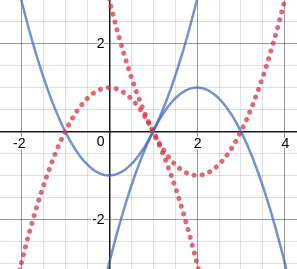
\includegraphics[scale=.3]{par1.png}
\caption{Possible parabolas passing through $q=1$}
\label{fig:para1}
\end{figure}

\section{Algorithm}
In this section we provide the algorithms which have been used for solving this problem. Table 1 lists the algorithm flow for unsteady state analysis while table 2 provides the algorithm for steady state analysis.
\begin{table}[ht]
   \centering
   \sffamily
   \begin{tabular}{rlr}
     \rowcolor{black!75}
      \head{No.}& \head{Steps}  \\
     1 & Initialize $u$, $v$, $\psi$ and $\omega$ matrices        \\
     2 & Apply boundary conditions for $u$, $v$, $\psi$ and $\omega$ \\
     2 & Define the vorticity equation    \\
     3 & Solve Poisson equation for stream function    \\
     4 & Solve vorticity transport equation at a forward time step $t+\Delta t$ \\
     5 & Solve the Poisson equation for stream function at  $t+\Delta t$ by iterative method  \\
     6 & Find $u$ and $v$ using the vorticity function equation      \\
     7 & Check if the CFL criteria is satisified, if yes proced to next step     \\
     8 & Else change the time step size and repeat the loop     \\
  \end{tabular}
  \caption{Algorithm for Unsteady state analysis}
\end{table}

\begin{table}[ht]
   \centering
   \sffamily
   \begin{tabular}{rlr}
     \rowcolor{black!75}
      \head{No.}& \head{Steps}  \\
     1 & Initialize $u$, $v$, $\psi$ and $\omega$ matrices        \\
     2 & Apply boundary conditions for $u$, $v$, $\psi$ and $\omega$ \\
     2 & Define the vorticity equation    \\
     3 & Solve Poisson equation for stream function    \\
     4 & Solve vorticity transport equation at a forward time step $t+\Delta t$ \\
     5 & Solve the Poisson equation for stream function at  $t+\Delta t$ by iterative method  \\
     6 & Find $u$ and $v$ using the vorticity function equation      \\
     7 & Check if the CFL criteria is satisified, if yes proced to next step     \\
     8 & Else change the time step size and repeat the loop     \\
  \end{tabular}
  \caption{Algorithm for Steady state analysis}
\end{table}



\section{Results}
% what is the Re at which turbulance starts and fluid shows transition i.e. vorticities

\subsection{Grid Independence Studies}

\subsection{Streamlines for Varying R and Re}

\subsection{Profiles for Steady Flow}

\section{Discussion}
Exact Fermi Dirac Integral expressions can be very helpful in generalizing the Wiedemann Franz  Law. Exact analytic expressions of the same will greatly assist and equip the researchers in the new material design processes.  Electronic thermal conductivity, $\kappa_e$ and minimum lattice thermal conductivity $\kappa_{l,min}$  have exact analytic expressions and we have obtained very interesting forms of solutions while maximising the two. More recent observations on the influence of anharmonicity on  $\kappa_{l,min}$  suggest that the Polylogarithms and Lambert W can have more interesting applications.

\section*{Appendix A}
Algorithm implimentation for unsteady state.
\lstinputlisting{71.py}

\section*{Appendix B}
Algorithm implimentation for steady state.
\lstinputlisting{73n.py}

\section*{Appendix C}
Algorithm implimentation for grid generation.
\lstinputlisting{gridGen.py}

\bibliographystyle{plain}
\bibliography{references}
\end{document}

